%
% main.tex -- Paper zum Thema <punktgruppen>
%
% (c) 2020 Hochschule Rapperswil
%
\chapter{Crystal M\rotatebox[origin=c]{180}{a}th\label{chapter:punktgruppen}}
\lhead{Crystal M\rotatebox[origin=c]{180}{a}th}
\begin{refsection}
\chapterauthor{Tim T\"onz, Naoki Pross}

%
% intro.tex
%
% (c) 2020 Prof Dr Andreas Müller, Hochschule Rapperswil
%
\bgroup

\definecolor{darkgreen}{rgb}{0,0.6,0}
\def\r{4}

\def\rad#1{
\begin{scope}[rotate=#1]
\fill[color=blue!20] (0,0) -- (-60:\r) arc (-60:60:\r) -- cycle;
\fill[color=darkgreen!20] (0,0) -- (60:\r) arc (60:180:\r) -- cycle;
\fill[color=orange!20] (0,0) -- (180:\r) arc (180:300:\r) -- cycle;

\node[color=darkgreen] at (120:3.7) [rotate={#1+30}] {Algebra};
\node[color=orange] at (240:3.7) [rotate={#1+150}] {Analysis};
\node[color=blue] at (0:3.7) [rotate={#1-90}] {Zerlegung};
\end{scope}
}

\begin{frame}
\frametitle{Intro --- Matrizen}

\vspace{-25pt}
\begin{center}
\begin{tikzpicture}[>=latex,thick]

\only<1-8>{
	\rad{-30}
	\only<2->{ \node at (90:3.0) {Rechenregeln $A^2+A+I=0$}; }
	\only<3->{ \node at (90:2.5) {Polynome $\chi_A(A)=0$, $m_A(A)=0$}; }
	\only<4->{ \node at (90:2.0) {Projektion: $P^2=P$}; }
	\only<5->{ \node at (90:1.5) {nilpotent: $N^k=0$}; }
}

\only<9-14>{
	\rad{90}
	\only<10->{ \node at (90:2.7) {Eigenbasis: $A=\sum \lambda_k P_k$}; }
	\only<11->{ \node at (90:2.2) {Invariante Räume:
		$AV\subset V, AV^\perp\subset V^\perp$}; }
}

\only<15-22>{
	\rad{210}
	\only<16->{ \node at (90:3.3) {Symmetrien}; }
	\only<17->{ \node at (90:2.8) {Skalarprodukt erhalten:
		$\operatorname{SO}(n)$}; }
	\only<18->{ \node at (90:2.3) {Konstant $\Rightarrow$ Ableitung $=0$}; }
	\only<19->{ \node at (90:1.5) {$\displaystyle \exp(A)
		= \sum_{k=0}^\infty \frac{A^k}{k!}$};
	}
}

\fill[color=red!20] (0,0) circle[radius=1.0];
\node at (0,0.25) {Matrizen};
\node at (0,-0.25) {$M_{m\times n}(\Bbbk)$};

\uncover<6->{
	\node[color=darkgreen] at (4.3,3.4) [right] {Algebra};
	\node at (4.3,2.2) [right] {\begin{minipage}{5cm}
	\begin{itemize}
	\item<6-> Algebraische Strukturen
	\item<7-> Polynome, Teilbarkeit
	\item<8-> Minimalpolynom
	\end{itemize}
	\end{minipage}};
}

\uncover<12->{
	\node[color=blue] at (4.3,0.8) [right] {Zerlegung};
	\node at (4.3,-0.4) [right] {\begin{minipage}{5cm}
	\begin{itemize}
	\item<12-> Eigenvektoren, -räume
	\item<13-> Projektionen, Drehungen
	\item<14-> Invariante Unterräume
	\end{itemize}
	\end{minipage}};
}

\uncover<20->{
	\node[color=orange] at (4.3,-1.8) [right] {Analysis};
	\node at (4.3,-3.0) [right] {\begin{minipage}{6cm}
	\begin{itemize}
	\item<20-> Symmetrien
	\item<21-> Matrix-DGL
	\item<22-> Matrix-Potenzreihen
	\end{itemize}
	\end{minipage}};
}

\end{tikzpicture}
\end{center}

\end{frame}

\egroup

\section{Symmetrie}
Das Wort Symmetrie ist sehr alt und hat sich seltsamerweise von seinem
ursprünglichen griechischen Wort
\(\mathrm{\sigma\nu\mu\mu\varepsilon\tau\rho\iota\alpha}\)
\footnote{\emph{Simmetr\'ia}: ein gemeinsames Mass habend, gleichmässig,
verhältnismässig} fast nicht verändert. In der Alltagssprache mag es ein
locker definierter Begriff sein, aber in der Mathematik hat Symmetrie eine sehr
präzise Bedeutung.
\begin{definition}[Symmetrie]
	Ein mathematisches Objekt wird als symmetrisch bezeichnet, wenn es unter einer
	bestimmten Operation invariant ist.
\end{definition}

Wenn der Leser noch nicht mit der Gruppentheorie in Berührung gekommen ist, ist
vielleicht nicht ganz klar, was eine Operation ist, aber die Definition sollte
trotzdem Sinn machen. Die Formalisierung dieser Idee wird bald kommen, aber
zunächst wollen wir eine Intuition aufbauen.

\begin{figure}[h]
	\centering
	\begin{tikzpicture}[
			node distance = 2cm,
			shapetheme/.style = {
				very thick, draw = black, fill = magenta!20!white,
				minimum size = 2cm,
			},
			line/.style = {thick, draw = darkgray},
			axis/.style = {line, dashed},
			dot/.style = {
				circle, draw = darkgray, fill = darkgray,
				minimum size = 1mm, inner sep = 0, outer sep = 0,
			},
		]

		\node[
			shapetheme,
			rectangle
		] (R) {};
		\node[dot] at (R) {};
		\draw[axis] (R) ++(-1.5, 0) to ++(3, 0) node[right] {\(\sigma\)};

		\node[
			shapetheme,
			regular polygon,
			regular polygon sides = 5,
			right = of R,
		] (Ps) {};
		\node[dot] (P) at (Ps) {};
		\draw[line, dotted] (P) to ++(18:1.5);
		\draw[line, dotted] (P) to ++(90:1.5);
		\draw[line, ->] (P) ++(18:1.2) 
			arc (18:90:1.2) node[midway, above right] {\(r, 72^\circ\)};

		\node[
			shapetheme,
			circle, right = of P
		] (Cs) {};
		\node[dot] (C) at (Cs) {};
		\draw[line, dotted] (C) to ++(1.5,0);
		\draw[line, dotted] (C) to ++(60:1.5);
		\draw[line, ->] (C) ++(1.2,0)
			arc (0:60:1.2) node[midway, above right] {\(r, \alpha\)};

	\end{tikzpicture}
	\caption{
		Beispiele für geometrisch symmetrische Formen.
		\label{fig:punktgruppen:geometry-example}
	}
\end{figure}

Die intuitivsten Beispiele kommen aus der Geometrie, daher werden wir mit
einigen geometrischen Beispielen beginnen. Wie wir jedoch später sehen werden,
ist das Konzept der Symmetrie eigentlich viel allgemeiner.  In Abbildung
\ref{fig:punktgruppen:geometry-example} haben wir einige Formen, die
offensichtlich symmetrisch sind.  Zum Beispiel hat ein Quadrat viele Achsen, um
die es gedreht werden kann, ohne sein Aussehen zu verändern.  Regelmässige
Polygone mit \(n\) Seiten sind gute Beispiele, um eine diskrete
Rotationssymmetrie zu veranschaulichen, was bedeutet, dass eine Drehung um
einen Punkt um einen bestimmten Winkel \(360^\circ/n\) sie unverändert lässt.
Das letzte Beispiel auf der rechten Seite ist eine unendliche
Rotationssymmetrie. Sie wird so genannt, weil es unendlich viele Werte für
\(\alpha \in \mathbb{R}\) gibt, die die Form unverändert lassen.  Dies ist
hoffentlich ausreichend, um die Bedeutung hinter der Notation zu verstehen, die
nun eingeführt wird.

\begin{definition}[Symmetriegruppe]
	Sei \(g\) eine Operation, die ein mathematisches Objekt unverändert lässt.
	Bei einer anderen Operation \(h\) definieren wir die Komposition \(h\circ g\)
	als die Anwendung der Operationen nacheinander. Alle Operationen bilden unter
	Komposition eine Gruppe, die Symmetriegruppe genannt wird.
\end{definition}

Mit dem oben Gesagten können wir das \(n\)-Gon Beispiel formalisieren. Wenn wir
\(r\) eine Drehung von \(2\pi/n\) sein lassen, gibt es eine wohlbekannte Symmetriegruppe
\[
	C_n = \langle r \rangle
		= \left\{\mathds{1}, r, r^2, \ldots, r^{n-1}\right\}
		= \mathbb{Z}/n\mathbb{Z},
\]
die Zyklische Gruppe heisst. Hier die Potenzen von \(r\) sind als wiederholte
Komposition gemeint, d.h. \(r^n = r\circ r \circ \cdots r\circ r\).  Die
Schreibweise mit den spitzen Klammern wird als Erzeugendensystem bezeichnet.
Das liegt daran, dass alle Elemente der Symmetriegruppe aus Kombinationen einer
Teilmenge erzeugt werden, die als erzeugende Elemente bezeichnet werden.  Die
Reflexionssymmetriegruppe ist nicht so interessant, da sie nur
\(\left\{\mathds{1}, \sigma\right\}\) enthält. Kombiniert man sie jedoch mit
der Rotation, erhält man die so genannte Diedergruppe
\[
	D_n = \langle r, \sigma : r^{n-1} = \sigma^2 = (\sigma r)^2 = \mathds{1} \rangle
		= \left\{
				\mathds{1}, r, \ldots, r^{n-1}, \sigma, \sigma r, \ldots, \sigma r^{n-1}
		\right\}.
\]
Diesmal muss die Generator-Notation die Beziehungen zwischen den beiden
Operationen beinhalten. Die ersten beiden sind leicht zu erkennen, für die
letzte empfehlen wir, sie an einem 2D-Quadrat auszuprobieren.

Wir haben nun unseren Operationen Symbole gegeben, mit denen es tatsächlich
möglich ist, eine nicht kommutative Algebra zu erstellen. Die naheliegende
Frage ist dann, könnte es sein, dass wir bereits etwas haben, das dasselbe tut?
Natürlich, ja. Dafür führen wir den Begriff der Darstellung ein.
\begin{definition}[Darstellung einer Gruppe, Gruppenhomomorphismus]
	Seien \(G\) und \(H\) Gruppe mit unterschiedlicher Operation \(\diamond\)
	bzw.  \(\star\). Ein Homomorphismus\footnote{ Für eine ausführlichere
	Diskussion siehe \S\ref{buch:grundlagen:subsection:gruppen} im Buch.} ist
	eine Funktion \(f: G \to H\), so dass für jedes \(a, b \in G\) gilt
	\(f(a\diamond b) = f(a) \star f(b)\).  Man sagt, dass der Homomorphismus
	\(f\) \(G\) in \(H\) transformiert, oder dass \(H\) eine Darstellung von
	\(G\) ist.
\end{definition}
\begin{beispiel}
	Die Elemente \(r^k \in C_n\), wobei \(0 < k < n\), stellen abstrakt eine
	Drehung von \(2\pi k/n\) um den Ursprung dar. Die mit der Matrix 
	\[
		\Phi(r^k) = \begin{pmatrix}
			\cos(2\pi k/n) & -\sin(2\pi k/n) \\
			\sin(2\pi k/n) &  \cos(2\pi k/n)
		\end{pmatrix}
	\]
	definierte Funktion von \(C_n\) nach \(O(2)\) ist eine Darstellung von
	\(C_n\). In diesem Fall ist die erste Gruppenoperation die Komposition und
	die zweite die Matrixmultiplikation. Man kann überprüfen, dass \(\Phi(r^2
	\circ r) = \Phi(r^2)\Phi(r)\).
\end{beispiel}
\begin{beispiel}
	Die Rotationssymmetrie des Kreises \(C_\infty\), mit einem unendlichen
	Kontinuum von Werten \(\alpha \in \mathbb{R}\), entspricht perfekt dem
	komplexen Einheitskreis. Der Homomorphismus \(\phi: C_\infty \to \mathbb{C}\)
	ist durch die Eulersche Formel \(\phi(r) = e^{i\alpha}\) gegeben.
\end{beispiel}

Die Symmetrien, die wir bis jetzt besprochen haben, haben immer mindestens
einen Punkt unbesetzt gelassen. Im Fall der Rotation war es der Drehpunkt, bei
der Spiegelung die Achse. Dies ist jedoch keine Voraussetzung für eine
Symmetrie, da es Symmetrien gibt, die jeden Punkt zu einem anderen Punkt
verschieben können. Ein aufmerksamer Leser wird bemerken, dass die
unveränderten Punkte zum Eigenraum\footnote{Zur Erinnerung \(E_\lambda =
\mathrm{null}(\Phi - \lambda I)\), \(\vec{v}\in E_\lambda \implies \Phi \vec{v}
= \lambda\vec{v}\)} der Matrixdarstellung der Symmetrieoperation gehören.
Diesen Spezialfall, bei dem mindestens ein Punkt unverändert bleibt, nennt man
Punktsymmetrie.
\begin{definition}[Punktgruppe]
	Wenn jede Operation in einer Symmetriegruppe die Eigenschaft hat, mindestens
	einen Punkt unverändert zu lassen, sagt man, dass die Symmetriegruppe eine
	Punktgruppe ist.
\end{definition}
Um das Konzept zu illustrieren, werden wir den umgekehrten Fall diskutieren:
eine Symmetrie, die keine Punktsymmetrie ist, die aber in der Physik sehr
nützlich ist, nämlich die Translationssymmetrie.  Von einem mathematischen
Objekt \(U\) wird gesagt, dass es eine Translationssymmetrie \(Q(x) = x + a\)
hat, wenn es die Gleichung 
\[
	U(x) = U(Q(x)) = U(x + a),
\]
für ein gewisses \(a\), erfüllt. Zum Beispiel besagt das erste Newtonsche
Gesetz, dass ein Objekt, auf das keine Kraft einwirkt, eine
zeitranslationsinvariante Geschwindigkeit hat, d.h. wenn \(\vec{F} = \vec{0}\)
dann \(\vec{v}(t) = \vec{v}(t + \tau)\).

% \subsection{Sch\"onflies notation} 

% vim:ts=2 sw=2 spell spelllang=de:

\section{Kristalle}
Unter dem Begriff Kristall sollte sich jeder ein Bild machen können. 
Wir werden uns aber nicht auf sein Äusseres fokussieren, sondern was ihn im Inneren ausmacht.
Die Innereien eines Kristalles sind glücklicherweise relativ einfach definiert.
\begin{definition}[Kristall]
    Ein Kristall besteht aus Atomen, welche sich in einem Muster arrangieren, welches sich in drei Dimensionen periodisch wiederholt.
\end{definition}


Ein Zweidimensionales Beispiel eines solchen Muster ist Abbildung \ref{fig:punktgruppen:lattce-grid}.
Für die Überschaubarkeit haben wir ein simples Muster eines einzelnen XgrauenX Punktes gewählt in nur Zwei Dimensionen.
Die eingezeichneten Vektoren a und b sind die kleinstmöglichen Schritte im Raum bis sich das Kristallgitter wiederholt.
Dadurch können von einem einzelnen XGrauenX Gitterpunkt in \ref{fig:punktgruppen:lattce-grid} können mit einer ganzzahligen Linearkombination von a und b alle anderen Gitterpunkte des Kristalles erreicht werden.
Ein Kristallgitter kann eindeutig mit a und b und deren winkeln beschrieben werden weswegen a und b auch Gitterparameter genannt werden.
Im Dreidimensionalen-Raum können alle Gitterpunkte mit derselben Idee und einem zusätzlichen Vektor also FRMEL FÜR TRANSLATIONSVEKTOR  erreicht werden.
Da sich das Ganze Kristallgitter wiederholt, wiederholen sich auch die Eigenschaften eines Gitterpunktes Periodisch mit eiem

\section{Piezoelektrizit\"at}


\nocite{punktgruppen:pinter-algebra}
\nocite{punktgruppen:sands-crystal}
\nocite{punktgruppen:lang-elt2}

\printbibliography[heading=subbibliography]
\end{refsection}
